\noindent\resizebox{0.6\textwidth}{!}{




\tikzset{every picture/.style={line width=0.75pt}} %set default line width to 0.75pt        

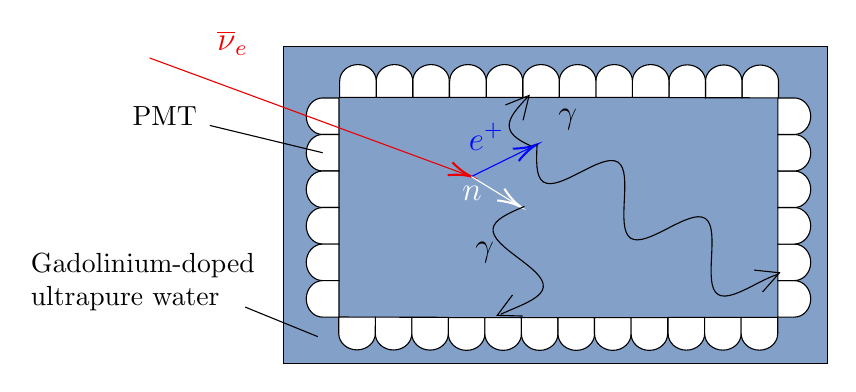
\begin{tikzpicture}[x=0.75pt,y=0.75pt,yscale=-1,xscale=1]
%uncomment if require: \path (0,300); %set diagram left start at 0, and has height of 300

%Shape: Rectangle [id:dp018761567314860672] 
\draw  [fill={rgb, 255:red, 131; green, 160; blue, 201 }  ,fill opacity=1 ] (180.88,72.3) -- (443.03,72.3) -- (443.03,224.8) -- (180.88,224.8) -- cycle ;
%Flowchart: Delay [id:dp3453792249551574] 
\draw  [fill={rgb, 255:red, 255; green, 255; blue, 255 }  ,fill opacity=1 ] (419.2,185) -- (427.1,185) .. controls (431.46,185) and (435,188.94) .. (435,193.8) .. controls (435,198.66) and (431.46,202.6) .. (427.1,202.6) -- (419.2,202.6) -- cycle ;
%Flowchart: Delay [id:dp4968083597677997] 
\draw  [fill={rgb, 255:red, 255; green, 255; blue, 255 }  ,fill opacity=1 ] (419.2,167.4) -- (427.1,167.4) .. controls (431.46,167.4) and (435,171.34) .. (435,176.2) .. controls (435,181.06) and (431.46,185) .. (427.1,185) -- (419.2,185) -- cycle ;
%Flowchart: Delay [id:dp21222118304763304] 
\draw  [fill={rgb, 255:red, 255; green, 255; blue, 255 }  ,fill opacity=1 ] (419.2,149.8) -- (427.1,149.8) .. controls (431.46,149.8) and (435,153.74) .. (435,158.6) .. controls (435,163.46) and (431.46,167.4) .. (427.1,167.4) -- (419.2,167.4) -- cycle ;

%Flowchart: Delay [id:dp12543071088571667] 
\draw  [fill={rgb, 255:red, 255; green, 255; blue, 255 }  ,fill opacity=1 ] (419.2,132.2) -- (427.1,132.2) .. controls (431.46,132.2) and (435,136.14) .. (435,141) .. controls (435,145.86) and (431.46,149.8) .. (427.1,149.8) -- (419.2,149.8) -- cycle ;
%Flowchart: Delay [id:dp5400522434110087] 
\draw  [fill={rgb, 255:red, 255; green, 255; blue, 255 }  ,fill opacity=1 ] (419.2,114.6) -- (427.1,114.6) .. controls (431.46,114.6) and (435,118.54) .. (435,123.4) .. controls (435,128.26) and (431.46,132.2) .. (427.1,132.2) -- (419.2,132.2) -- cycle ;
%Flowchart: Delay [id:dp484150119956154] 
\draw  [fill={rgb, 255:red, 255; green, 255; blue, 255 }  ,fill opacity=1 ] (419.2,97) -- (427.1,97) .. controls (431.46,97) and (435,100.94) .. (435,105.8) .. controls (435,110.66) and (431.46,114.6) .. (427.1,114.6) -- (419.2,114.6) -- cycle ;


%Flowchart: Delay [id:dp9023215219964117] 
\draw  [fill={rgb, 255:red, 255; green, 255; blue, 255 }  ,fill opacity=1 ] (401.88,96.92) -- (401.9,89.02) .. controls (401.91,84.66) and (405.86,81.14) .. (410.72,81.15) .. controls (415.58,81.16) and (419.51,84.71) .. (419.5,89.07) -- (419.48,96.97) -- cycle ;
%Flowchart: Delay [id:dp8855637019163796] 
\draw  [fill={rgb, 255:red, 255; green, 255; blue, 255 }  ,fill opacity=1 ] (384.28,96.88) -- (384.3,88.98) .. controls (384.31,84.61) and (388.26,81.09) .. (393.12,81.1) .. controls (397.98,81.11) and (401.91,84.66) .. (401.9,89.02) -- (401.88,96.92) -- cycle ;
%Flowchart: Delay [id:dp15396139910681717] 
\draw  [fill={rgb, 255:red, 255; green, 255; blue, 255 }  ,fill opacity=1 ] (366.68,96.83) -- (366.7,88.93) .. controls (366.71,84.56) and (370.66,81.04) .. (375.52,81.05) .. controls (380.38,81.06) and (384.31,84.61) .. (384.3,88.98) -- (384.28,96.88) -- cycle ;

%Flowchart: Delay [id:dp9341704555928705] 
\draw  [fill={rgb, 255:red, 255; green, 255; blue, 255 }  ,fill opacity=1 ] (349.1,96.72) -- (349.1,88.82) .. controls (349.1,84.46) and (353.04,80.92) .. (357.9,80.92) .. controls (362.76,80.92) and (366.7,84.46) .. (366.7,88.82) -- (366.7,96.72) -- cycle ;
%Flowchart: Delay [id:dp35133572705603155] 
\draw  [fill={rgb, 255:red, 255; green, 255; blue, 255 }  ,fill opacity=1 ] (331.5,96.72) -- (331.5,88.82) .. controls (331.5,84.46) and (335.44,80.92) .. (340.3,80.92) .. controls (345.16,80.92) and (349.1,84.46) .. (349.1,88.82) -- (349.1,96.72) -- cycle ;
%Flowchart: Delay [id:dp21764093907647952] 
\draw  [fill={rgb, 255:red, 255; green, 255; blue, 255 }  ,fill opacity=1 ] (313.9,96.72) -- (313.9,88.82) .. controls (313.9,84.46) and (317.84,80.92) .. (322.7,80.92) .. controls (327.56,80.92) and (331.5,84.46) .. (331.5,88.82) -- (331.5,96.72) -- cycle ;

%Flowchart: Delay [id:dp20972897669252522] 
\draw  [fill={rgb, 255:red, 255; green, 255; blue, 255 }  ,fill opacity=1 ] (296.26,96.72) -- (296.26,88.82) .. controls (296.26,84.46) and (300.2,80.92) .. (305.06,80.92) .. controls (309.92,80.92) and (313.86,84.46) .. (313.86,88.82) -- (313.86,96.72) -- cycle ;
%Flowchart: Delay [id:dp1550754280941704] 
\draw  [fill={rgb, 255:red, 255; green, 255; blue, 255 }  ,fill opacity=1 ] (278.66,96.72) -- (278.66,88.82) .. controls (278.66,84.46) and (282.6,80.92) .. (287.46,80.92) .. controls (292.32,80.92) and (296.26,84.46) .. (296.26,88.82) -- (296.26,96.72) -- cycle ;
%Flowchart: Delay [id:dp3988068800155561] 
\draw  [fill={rgb, 255:red, 255; green, 255; blue, 255 }  ,fill opacity=1 ] (261.06,96.72) -- (261.06,88.82) .. controls (261.06,84.46) and (265,80.92) .. (269.86,80.92) .. controls (274.72,80.92) and (278.66,84.46) .. (278.66,88.82) -- (278.66,96.72) -- cycle ;

%Flowchart: Delay [id:dp2664101802762959] 
\draw  [fill={rgb, 255:red, 255; green, 255; blue, 255 }  ,fill opacity=1 ] (383.9,202.7) -- (383.9,210.6) .. controls (383.9,214.96) and (379.96,218.5) .. (375.1,218.5) .. controls (370.24,218.5) and (366.3,214.96) .. (366.3,210.6) -- (366.3,202.7) -- cycle ;
%Flowchart: Delay [id:dp8686792133858285] 
\draw  [fill={rgb, 255:red, 255; green, 255; blue, 255 }  ,fill opacity=1 ] (401.5,202.7) -- (401.5,210.6) .. controls (401.5,214.96) and (397.56,218.5) .. (392.7,218.5) .. controls (387.84,218.5) and (383.9,214.96) .. (383.9,210.6) -- (383.9,202.7) -- cycle ;
%Flowchart: Delay [id:dp2917426852861188] 
\draw  [fill={rgb, 255:red, 255; green, 255; blue, 255 }  ,fill opacity=1 ] (419.1,202.7) -- (419.1,210.6) .. controls (419.1,214.96) and (415.16,218.5) .. (410.3,218.5) .. controls (405.44,218.5) and (401.5,214.96) .. (401.5,210.6) -- (401.5,202.7) -- cycle ;

%Flowchart: Delay [id:dp6716119172397017] 
\draw  [fill={rgb, 255:red, 255; green, 255; blue, 255 }  ,fill opacity=1 ] (242.83,202.65) -- (242.81,210.55) .. controls (242.8,214.92) and (238.85,218.44) .. (233.99,218.43) .. controls (229.13,218.41) and (225.2,214.87) .. (225.21,210.5) -- (225.23,202.6) -- cycle ;
%Flowchart: Delay [id:dp13338902682870213] 
\draw  [fill={rgb, 255:red, 255; green, 255; blue, 255 }  ,fill opacity=1 ] (260.43,202.7) -- (260.41,210.6) .. controls (260.4,214.96) and (256.45,218.49) .. (251.59,218.48) .. controls (246.73,218.46) and (242.8,214.92) .. (242.81,210.55) -- (242.83,202.65) -- cycle ;
%Flowchart: Delay [id:dp8307460210435487] 
\draw  [fill={rgb, 255:red, 255; green, 255; blue, 255 }  ,fill opacity=1 ] (278.01,202.81) -- (278.01,210.71) .. controls (278.01,215.07) and (274.07,218.61) .. (269.21,218.61) .. controls (264.35,218.61) and (260.41,215.07) .. (260.41,210.71) -- (260.41,202.81) -- cycle ;
%Flowchart: Delay [id:dp02162290080873741] 
\draw  [fill={rgb, 255:red, 255; green, 255; blue, 255 }  ,fill opacity=1 ] (295.61,202.81) -- (295.61,210.71) .. controls (295.61,215.07) and (291.67,218.61) .. (286.81,218.61) .. controls (281.95,218.61) and (278.01,215.07) .. (278.01,210.71) -- (278.01,202.81) -- cycle ;
%Flowchart: Delay [id:dp3989655724900727] 
\draw  [fill={rgb, 255:red, 255; green, 255; blue, 255 }  ,fill opacity=1 ] (313.21,202.81) -- (313.21,210.71) .. controls (313.21,215.07) and (309.27,218.61) .. (304.41,218.61) .. controls (299.55,218.61) and (295.61,215.07) .. (295.61,210.71) -- (295.61,202.81) -- cycle ;

%Flowchart: Delay [id:dp8387917491135258] 
\draw  [fill={rgb, 255:red, 255; green, 255; blue, 255 }  ,fill opacity=1 ] (330.85,202.81) -- (330.85,210.71) .. controls (330.85,215.07) and (326.91,218.61) .. (322.05,218.61) .. controls (317.19,218.61) and (313.25,215.07) .. (313.25,210.71) -- (313.25,202.81) -- cycle ;
%Flowchart: Delay [id:dp02844567706050738] 
\draw  [fill={rgb, 255:red, 255; green, 255; blue, 255 }  ,fill opacity=1 ] (348.45,202.81) -- (348.45,210.71) .. controls (348.45,215.07) and (344.51,218.61) .. (339.65,218.61) .. controls (334.79,218.61) and (330.85,215.07) .. (330.85,210.71) -- (330.85,202.81) -- cycle ;
%Flowchart: Delay [id:dp018274983277363654] 
\draw  [fill={rgb, 255:red, 255; green, 255; blue, 255 }  ,fill opacity=1 ] (366.05,202.81) -- (366.05,210.71) .. controls (366.05,215.07) and (362.11,218.61) .. (357.25,218.61) .. controls (352.39,218.61) and (348.45,215.07) .. (348.45,210.71) -- (348.45,202.81) -- cycle ;

%Flowchart: Delay [id:dp11642740678628094] 
\draw  [fill={rgb, 255:red, 255; green, 255; blue, 255 }  ,fill opacity=1 ] (225.23,202.6) -- (225.21,210.5) .. controls (225.2,214.87) and (221.25,218.39) .. (216.39,218.38) .. controls (211.53,218.37) and (207.6,214.82) .. (207.61,210.45) -- (207.63,202.55) -- cycle ;

%Flowchart: Delay [id:dp2633719534438189] 
\draw  [fill={rgb, 255:red, 255; green, 255; blue, 255 }  ,fill opacity=1 ] (207.75,114.6) -- (199.85,114.6) .. controls (195.49,114.6) and (191.95,110.66) .. (191.95,105.8) .. controls (191.95,100.94) and (195.49,97) .. (199.85,97) -- (207.75,97) -- cycle ;
%Flowchart: Delay [id:dp6972124496267963] 
\draw  [fill={rgb, 255:red, 255; green, 255; blue, 255 }  ,fill opacity=1 ] (207.75,132.2) -- (199.85,132.2) .. controls (195.49,132.2) and (191.95,128.26) .. (191.95,123.4) .. controls (191.95,118.54) and (195.49,114.6) .. (199.85,114.6) -- (207.75,114.6) -- cycle ;
%Flowchart: Delay [id:dp5081089105018392] 
\draw  [fill={rgb, 255:red, 255; green, 255; blue, 255 }  ,fill opacity=1 ] (207.75,149.8) -- (199.85,149.8) .. controls (195.49,149.8) and (191.95,145.86) .. (191.95,141) .. controls (191.95,136.14) and (195.49,132.2) .. (199.85,132.2) -- (207.75,132.2) -- cycle ;

%Flowchart: Delay [id:dp8541254717293781] 
\draw  [fill={rgb, 255:red, 255; green, 255; blue, 255 }  ,fill opacity=1 ] (207.75,167.4) -- (199.85,167.4) .. controls (195.49,167.4) and (191.95,163.46) .. (191.95,158.6) .. controls (191.95,153.74) and (195.49,149.8) .. (199.85,149.8) -- (207.75,149.8) -- cycle ;
%Flowchart: Delay [id:dp8530575300066843] 
\draw  [fill={rgb, 255:red, 255; green, 255; blue, 255 }  ,fill opacity=1 ] (207.75,185) -- (199.85,185) .. controls (195.49,185) and (191.95,181.06) .. (191.95,176.2) .. controls (191.95,171.34) and (195.49,167.4) .. (199.85,167.4) -- (207.75,167.4) -- cycle ;
%Flowchart: Delay [id:dp6996814816352454] 
\draw  [fill={rgb, 255:red, 255; green, 255; blue, 255 }  ,fill opacity=1 ] (207.75,202.6) -- (199.85,202.6) .. controls (195.49,202.6) and (191.95,198.66) .. (191.95,193.8) .. controls (191.95,188.94) and (195.49,185) .. (199.85,185) -- (207.75,185) -- cycle ;


%Flowchart: Delay [id:dp059593379898308374] 
\draw  [fill={rgb, 255:red, 255; green, 255; blue, 255 }  ,fill opacity=1 ] (243.26,96.72) -- (243.26,88.82) .. controls (243.26,84.46) and (247.2,80.92) .. (252.06,80.92) .. controls (256.92,80.92) and (260.86,84.46) .. (260.86,88.82) -- (260.86,96.72) -- cycle ;
%Flowchart: Delay [id:dp032634547707062755] 
\draw  [fill={rgb, 255:red, 255; green, 255; blue, 255 }  ,fill opacity=1 ] (225.66,96.72) -- (225.66,88.82) .. controls (225.66,84.46) and (229.6,80.92) .. (234.46,80.92) .. controls (239.32,80.92) and (243.26,84.46) .. (243.26,88.82) -- (243.26,96.72) -- cycle ;
%Flowchart: Delay [id:dp47193256820467144] 
\draw  [fill={rgb, 255:red, 255; green, 255; blue, 255 }  ,fill opacity=1 ] (208.06,96.72) -- (208.06,88.82) .. controls (208.06,84.46) and (212,80.92) .. (216.86,80.92) .. controls (221.72,80.92) and (225.66,84.46) .. (225.66,88.82) -- (225.66,96.72) -- cycle ;

%Straight Lines [id:da18093906247709823] 
\draw [color={rgb, 255:red, 235; green, 1; blue, 1 }  ,draw opacity=1 ]   (116.5,77.75) -- (269.62,134.18) ;
\draw [shift={(271.5,134.88)}, rotate = 200.23] [color={rgb, 255:red, 235; green, 1; blue, 1 }  ,draw opacity=1 ][line width=0.75]    (10.93,-3.29) .. controls (6.95,-1.4) and (3.31,-0.3) .. (0,0) .. controls (3.31,0.3) and (6.95,1.4) .. (10.93,3.29)   ;
%Straight Lines [id:da1327149906789582] 
\draw [color={rgb, 255:red, 0; green, 6; blue, 255 }  ,draw opacity=1 ][fill={rgb, 255:red, 6; green, 37; blue, 244 }  ,fill opacity=1 ]   (271.5,134.88) -- (300.92,120.45) ;
\draw [shift={(302.71,119.57)}, rotate = 513.88] [color={rgb, 255:red, 0; green, 6; blue, 255 }  ,draw opacity=1 ][line width=0.75]    (10.93,-3.29) .. controls (6.95,-1.4) and (3.31,-0.3) .. (0,0) .. controls (3.31,0.3) and (6.95,1.4) .. (10.93,3.29)   ;
%Straight Lines [id:da41117101424092894] 
\draw [color={rgb, 255:red, 255; green, 255; blue, 255 }  ,draw opacity=1 ][fill={rgb, 255:red, 199; green, 201; blue, 213 }  ,fill opacity=1 ]   (271.5,134.88) -- (293.3,148.24) ;
\draw [shift={(295,149.29)}, rotate = 211.52] [color={rgb, 255:red, 255; green, 255; blue, 255 }  ,draw opacity=1 ][line width=0.75]    (10.93,-3.29) .. controls (6.95,-1.4) and (3.31,-0.3) .. (0,0) .. controls (3.31,0.3) and (6.95,1.4) .. (10.93,3.29)   ;
%Straight Lines [id:da23289309495912702] 
\draw    (162.5,197.75) -- (197.5,212) ;
%Straight Lines [id:da35705856166793093] 
\draw    (145.5,110.25) -- (199.85,123.4) ;
%Shape: Wave [id:dp9780044910616013] 
\draw   (297.09,149.25) .. controls (289.62,152.44) and (282.5,155.49) .. (281.95,159.98) .. controls (281.4,164.47) and (287.56,169.16) .. (294.05,174.06) .. controls (300.53,178.97) and (306.7,183.65) .. (306.15,188.14) .. controls (305.6,192.63) and (298.48,195.69) .. (291,198.88) .. controls (289.15,199.66) and (287.33,200.44) .. (285.62,201.24) ;
\draw   (296.24,202.07) -- (283.96,201.76) -- (291.32,191.93) ;
%Shape: Wave [id:dp12522818071488817] 
\draw   (303.17,119.17) .. controls (302.79,127.29) and (302.44,135.03) .. (306.24,137.48) .. controls (310.05,139.93) and (316.95,136.42) .. (324.19,132.72) .. controls (331.42,129.01) and (338.33,125.5) .. (342.13,127.95) .. controls (345.93,130.4) and (345.58,138.14) .. (345.2,146.26) .. controls (344.82,154.38) and (344.47,162.12) .. (348.27,164.57) .. controls (352.08,167.02) and (358.98,163.5) .. (366.21,159.8) .. controls (373.45,156.1) and (380.35,152.59) .. (384.16,155.04) .. controls (387.96,157.49) and (387.61,165.23) .. (387.23,173.34) .. controls (386.85,181.46) and (386.5,189.2) .. (390.3,191.65) .. controls (394.1,194.1) and (401.01,190.59) .. (408.24,186.89) .. controls (411.97,184.98) and (415.61,183.12) .. (418.79,182.1) ;
\draw   (407.74,179.94) -- (419.95,181.23) -- (411.83,190.44) ;
%Shape: Wave [id:dp4888449474927056] 
\draw   (298.2,96.99) .. controls (293.45,102.09) and (288.93,106.97) .. (289.82,111.41) .. controls (290.56,115.11) and (294.89,117.65) .. (299.99,120.07) ;
\draw   (287.89,100.38) -- (299.3,95.83) -- (296.41,107.77) ;

% Text Node
\draw (147.83,63.41) node [anchor=north west][inner sep=0.75pt]  [font=\large,color={rgb, 255:red, 246; green, 0; blue, 0 }  ,opacity=1 ] [align=left] {$\displaystyle \overline{\nu }_{e}$};
% Text Node
\draw (312.13,101.27) node [anchor=north west][inner sep=0.75pt]  [font=\large,color={rgb, 255:red, 0; green, 0; blue, 0 }  ,opacity=1 ] [align=left] {$\displaystyle \gamma $};
% Text Node
\draw (272.21,165.07) node [anchor=north west][inner sep=0.75pt]  [font=\large,color={rgb, 255:red, 246; green, 0; blue, 0 }  ,opacity=1 ] [align=left] {\textcolor[rgb]{0,0,0}{$\displaystyle \gamma $}};
% Text Node
\draw (269.07,108) node [anchor=north west][inner sep=0.75pt]  [font=\large,color={rgb, 255:red, 11; green, 0; blue, 246 }  ,opacity=1 ] [align=left] {$\displaystyle \textcolor[rgb]{0,0.03,1}{e^{+}}$};
% Text Node
\draw (265.86,138.33) node [anchor=north west][inner sep=0.75pt]  [font=\large,color={rgb, 255:red, 246; green, 0; blue, 0 }  ,opacity=1 ] [align=left] {$\displaystyle \textcolor[rgb]{1,1,1}{n}$};
% Text Node
\draw (107,100) node [anchor=north west][inner sep=0.75pt]   [align=left] {PMT};
% Text Node
\draw (58,170.5) node [anchor=north west][inner sep=0.75pt]   [align=left] {Gadolinium-doped \\ultrapure water};


\end{tikzpicture}

}